% Created 2017-06-06 Tue 13:13
\documentclass[11pt]{article}
\usepackage[utf8]{inputenc}
\usepackage[T1]{fontenc}
\usepackage{fixltx2e}
\usepackage{graphicx}
\usepackage{longtable}
\usepackage{float}
\usepackage{wrapfig}
\usepackage{rotating}
\usepackage[normalem]{ulem}
\usepackage{amsmath}
\usepackage{textcomp}
\usepackage{marvosym}
\usepackage{wasysym}
\usepackage{amssymb}
\usepackage{hyperref}
\tolerance=1000
\author{Mehran}
\date{\today}
\title{gui\_design}
\hypersetup{
  pdfkeywords={},
  pdfsubject={},
  pdfcreator={Emacs 25.1.1 (Org mode 8.2.10)}}
\begin{document}

\maketitle
\tableofcontents

\section{Welcome screen:}
\label{sec-1}
\subsubsection{design:}
\label{sec-1-0-1}
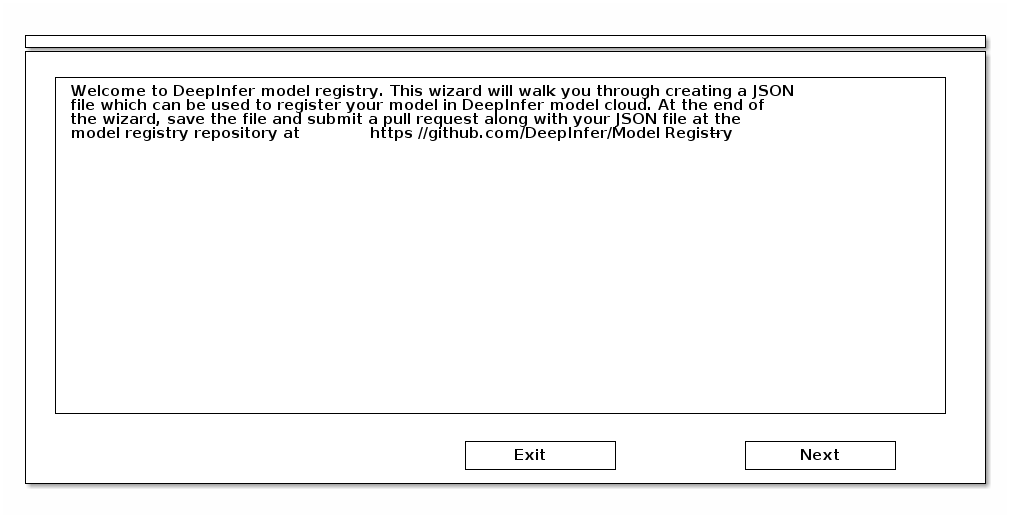
\includegraphics[width=.9\linewidth]{welcome.png}

\section{Model properties:}
\label{sec-2}
\subsubsection{name}
\label{sec-2-0-1}
\subsubsection{version}
\label{sec-2-0-2}
\subsubsection{task}
\label{sec-2-0-3}
\subsubsection{organ}
\label{sec-2-0-4}
\subsubsection{modality}
\label{sec-2-0-5}
\subsubsection{training data details}
\label{sec-2-0-6}
\subsubsection{description}
\label{sec-2-0-7}
\subsubsection{detailed description}
\label{sec-2-0-8}
\subsubsection{train:}
\label{sec-2-0-9}
\begin{enumerate}
\item number of subjects
\label{sec-2-0-9-1}
\end{enumerate}
\subsubsection{test:}
\label{sec-2-0-10}
\begin{enumerate}
\item number of subjects
\label{sec-2-0-10-1}
\item accuracy
\label{sec-2-0-10-2}
\item metric
\label{sec-2-0-10-3}
\end{enumerate}
\subsubsection{design:}
\label{sec-2-0-11}
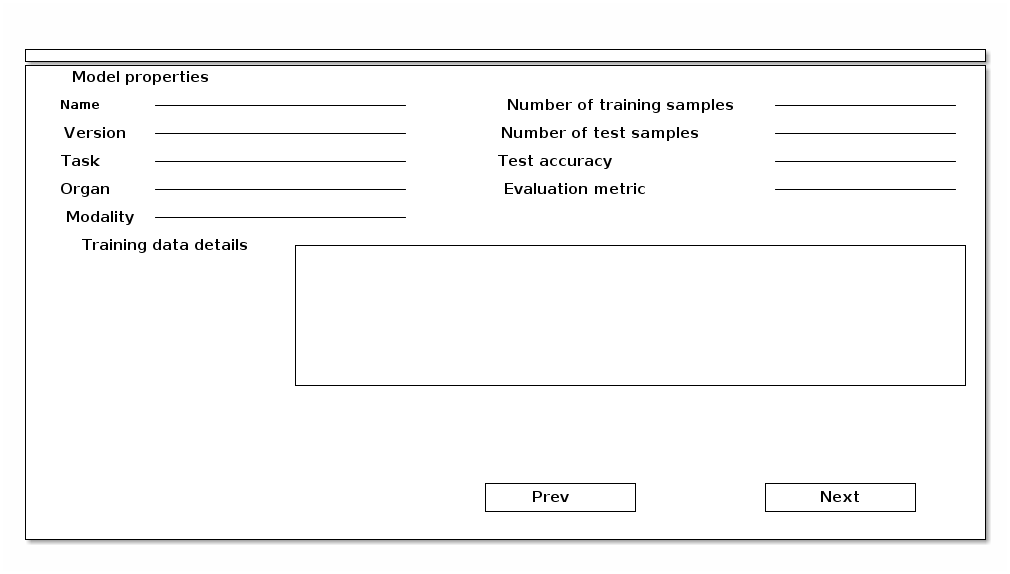
\includegraphics[width=.9\linewidth]{model-prop.png}

\section{Docker properties}
\label{sec-3}
\subsubsection{docker hub image}
\label{sec-3-0-1}
\subsubsection{digest}
\label{sec-3-0-2}
\subsubsection{size of the image}
\label{sec-3-0-3}
\subsubsection{design:}
\label{sec-3-0-4}
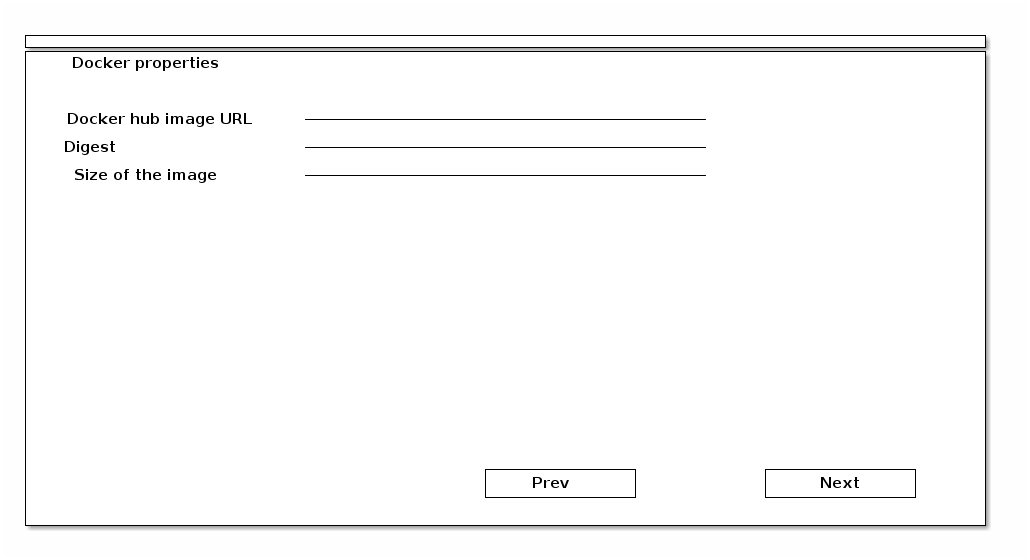
\includegraphics[width=.9\linewidth]{docker.png}
% Emacs 25.1.1 (Org mode 8.2.10)
\end{document}